% arara: xelatex
% arara: makeglossaries
% arara: xelatex
% arara: xelatex

% style inspired by
% https://github.com/omelkonian/presentations/blob/2c0b2e1f592a8f90797e4997c3ab8785b114f595/%5B2019.08.20%5D%20BitML%20(SRC%20Presentation%20@%20ICFP)/bitml-presentation.tex

\documentclass[aspectratio=169]{beamer}
\usetheme{metropolis}

\usepackage[utf8]{inputenc}
\usepackage[T1]{fontenc}
\usepackage{textcomp}
\usepackage[english]{babel}
\usepackage{amsmath, amssymb, bm}
\usepackage{tcolorbox}
\usepackage[makeroom]{cancel}
\usepackage{mathpartir}
\usepackage{xparse}

% for plotting data
\usepackage{pgfplotstable}
\usepackage{pgfplots}

% displayquote
\usepackage{csquotes}

% TikZ
\usepackage{tikz}
\usetikzlibrary{chains,arrows,automata,fit,positioning,calc}

% todos
\usepackage{todonotes}

% listings
\usepackage{listings}

% figure support
\usepackage{import}
\usepackage{xifthen}
\usepackage{pdfpages}
\usepackage{transparent}
\newcommand{\incfig}[1]{%
	\def\svgwidth{\columnwidth}
	\import{./figures/}{#1.pdf_tex}
}

% style for tcolorboxes
\tcbset{plain/.style={colbacktitle=white,coltitle=black,colback=white}}
\pdfsuppresswarningpagegroup=1

% fonts
\usepackage{relsize}
\usepackage[tt=false]{libertine}
\usepackage[libertine]{newtxmath}

% colours
\definecolor{CTUBlue}{HTML}{175BB0}
\setbeamercolor{alerted text}{fg=CTUBlue}


\title{P4 Language Server}
\author{Bc. Ondřej Kvapil\\ supervised by Ing. Viktor Puš, Ph.D., MBA}
\institute{Czech Technical University in Prague, Faculty of Information Technology}
\date{14th of June, 2023}


\begin{document}

\lstdefinelanguage{Rust}{%
  sensitive%
, morecomment=[l]{//}%
, morecomment=[s]{/*}{*/}%
, moredelim=[s][{\itshape\color[rgb]{0,0,0.75}}]{\#[}{]}%
, morestring=[b]{"}%
, alsodigit={}%
, alsoother={}%
, alsoletter={!}%
%
%
% [1] reserve keywords
% [2] traits
% [3] primitive types
% [4] type and value constructors
% [5] identifier
%
, morekeywords={break, continue, else, for, if, in, loop, match, return, while}
% control flow keywords
, morekeywords={as, const, let, move, mut, ref, static}  % in the context of variables
, morekeywords={dyn, enum, fn, impl, Self, self, struct, trait, type, union,
use, where}  % in the context of declarations
, morekeywords={crate, extern, mod, pub, super}  % in the context of
modularisation
, morekeywords={unsafe}  % markers
, morekeywords={abstract, alignof, become, box, do, final, macro, offsetof,
override, priv, proc, pure, sizeof, typeof, unsized, virtual, yield}  % reserved
identifiers
%
% grep 'pub trait [A-Za-z][A-Za-z0-9]*' -r . | sed 's/^.*pub trait \([A-Za-z][A-Za-z0-9]*\).*/\1/g' | sort -u | tr '\n' ',' | sed 's/^\(.*\),$/{\1}\n/g' | sed 's/,/, /g'
, morekeywords=[2]{Add, AddAssign, Any, AsciiExt, AsInner, AsInnerMut, AsMut,
AsRawFd, AsRawHandle, AsRawSocket, AsRef, Binary, BitAnd, BitAndAssign, Bitor,
BitOr, BitOrAssign, BitXor, BitXorAssign, Borrow, BorrowMut, Boxed, BoxPlace,
BufRead, BuildHasher, CastInto, CharExt, Clone, CoerceUnsized, CommandExt, Copy,
Debug, DecodableFloat, Default, Deref, DerefMut, DirBuilderExt, DirEntryExt,
Display, Div, DivAssign, DoubleEndedIterator, DoubleEndedSearcher, Drop, EnvKey,
Eq, Error, ExactSizeIterator, ExitStatusExt, Extend, FileExt, FileTypeExt,
Float, Fn, FnBox, FnMut, FnOnce, Freeze, From, FromInner, FromIterator,
FromRawFd, FromRawHandle, FromRawSocket, FromStr, FullOps, FusedIterator,
Generator, Hash, Hasher, Index, IndexMut, InPlace, Int, Into, IntoCow,
IntoInner, IntoIterator, IntoRawFd, IntoRawHandle, IntoRawSocket, IsMinusOne,
IsZero, Iterator, JoinHandleExt, LargeInt, LowerExp, LowerHex, MetadataExt, Mul,
MulAssign, Neg, Not, Octal, OpenOptionsExt, Ord, OsStrExt, OsStringExt, Packet,
PartialEq, PartialOrd, Pattern, PermissionsExt, Place, Placer, Pointer, Product,
Put, RangeArgument, RawFloat, Read, Rem, RemAssign, Seek, Shl, ShlAssign, Shr,
ShrAssign, Sized, SliceConcatExt, SliceExt, SliceIndex, Stats, Step, StrExt,
Sub, SubAssign, Sum, Sync, TDynBenchFn, Terminal, Termination, ToOwned,
ToSocketAddrs, ToString, Try, TryFrom, TryInto, UnicodeStr, Unsize, UpperExp,
UpperHex, WideInt, Write} , morekeywords=[2]{Send}  % additional traits
%
, morekeywords=[3]{bool, char, f32, f64, i8, i16, i32, i64, isize, str, u8, u16,
u32, u64, unit, usize, i128, u128}  % primitive types
%
, morekeywords=[4]{Err, false, None, Ok, Some, true}  % prelude value constructors
% grep 'pub \(type\|struct\|enum\) [A-Za-z][A-Za-z0-9]*' -r . | sed 's/^.*pub \(type\|struct\|enum\) \([A-Za-z][A-Za-z0-9]*\).*/\2/g' | sort -u | tr '\n' ',' | sed 's/^\(.*\),$/{\1}\n/g' | sed 's/,/, /g'
, morekeywords=[3]{AccessError, Adddf3, AddI128, AddoI128, AddoU128, ADDRESS,
ADDRESS64, addrinfo, ADDRINFOA, AddrParseError, Addsf3, AddU128, advice, aiocb,
Alignment, AllocErr, AnonPipe, Answer, Arc, Args, ArgsInnerDebug, ArgsOs,
Argument, Arguments, ArgumentV1, Ashldi3, Ashlti3, Ashrdi3, Ashrti3,
AssertParamIsClone, AssertParamIsCopy, AssertParamIsEq, AssertUnwindSafe,
AtomicBool, AtomicPtr, Attr, auxtype, auxv, BackPlace, BacktraceContext,
Barrier, BarrierWaitResult, Bencher, BenchMode, BenchSamples, BinaryHeap,
BinaryHeapPlace, blkcnt, blkcnt64, blksize, BOOL, boolean, BOOLEAN, BoolTrie,
BorrowError, BorrowMutError, Bound, Box, bpf, BTreeMap, BTreeSet, Bucket,
BucketState, Buf, BufReader, BufWriter, Builder, BuildHasherDefault, BY, BYTE,
Bytes, CannotReallocInPlace, cc, Cell, Chain, CHAR, CharIndices,
CharPredicateSearcher, Chars, CharSearcher, CharsError, CharSliceSearcher,
CharTryFromError, Child, ChildPipes, ChildStderr, ChildStdin, ChildStdio,
ChildStdout, Chunks, ChunksMut, ciovec, clock, clockid, Cloned, cmsgcred,
cmsghdr, CodePoint, Color, ColorConfig, Command, CommandEnv, Component,
Components, CONDITION, condvar, Condvar, CONSOLE, CONTEXT, Count, Cow, cpu,
CRITICAL, CStr, CString, CStringArray, Cursor, Cycle, CycleIter, daddr,
DebugList, DebugMap, DebugSet, DebugStruct, DebugTuple, Decimal, Decoded,
DecodeUtf16, DecodeUtf16Error, DecodeUtf8, DefaultEnvKey, DefaultHasher, dev,
device, Difference, Digit32, DIR, DirBuilder, dircookie, dirent, dirent64,
DirEntry, Discriminant, DISPATCHER, Display, Divdf3, Divdi3, Divmoddi4,
Divmodsi4, Divsf3, Divsi3, Divti3, dl, Dl, Dlmalloc, Dns, DnsAnswer, DnsQuery,
dqblk, Drain, DrainFilter, Dtor, Duration, DwarfReader, DWORD, DWORDLONG,
DynamicLibrary, Edge, EHAction, EHContext, Elf32, Elf64, Empty, EmptyBucket,
EncodeUtf16, EncodeWide, Entry, EntryPlace, Enumerate, Env, epoll, errno, Error,
ErrorKind, EscapeDebug, EscapeDefault, EscapeUnicode, event, Event,
eventrwflags, eventtype, ExactChunks, ExactChunksMut, EXCEPTION, Excess,
ExchangeHeapSingleton, exit, exitcode, ExitStatus, Failure, fd, fdflags,
fdsflags, fdstat, ff, fflags, File, FILE, FileAttr, filedelta, FileDesc,
FilePermissions, filesize, filestat, FILETIME, filetype, FileType, Filter,
FilterMap, Fixdfdi, Fixdfsi, Fixdfti, Fixsfdi, Fixsfsi, Fixsfti, Fixunsdfdi,
Fixunsdfsi, Fixunsdfti, Fixunssfdi, Fixunssfsi, Fixunssfti, Flag, FlatMap,
Floatdidf, FLOATING, Floatsidf, Floatsisf, Floattidf, Floattisf, Floatundidf,
Floatunsidf, Floatunsisf, Floatuntidf, Floatuntisf, flock, ForceResult,
FormatSpec, Formatted, Formatter, Fp, FpCategory, fpos, fpos64, fpreg, fpregset,
FPUControlWord, Frame, FromBytesWithNulError, FromUtf16Error, FromUtf8Error,
FrontPlace, fsblkcnt, fsfilcnt, fsflags, fsid, fstore, fsword, FullBucket,
FullBucketMut, FullDecoded, Fuse, GapThenFull, GeneratorState, gid, glob,
glob64, GlobalDlmalloc, greg, group, GROUP, Guard, GUID, Handle, HANDLE,
Handler, HashMap, HashSet, Heap, HINSTANCE, HMODULE, hostent, HRESULT, id,
idtype, if, ifaddrs, IMAGEHLP, Immut, in, in6, Incoming, Infallible,
Initializer, ino, ino64, inode, input, InsertResult, Inspect, Instant, int16,
int32, int64, int8, integer, IntermediateBox, Internal, Intersection, intmax,
IntoInnerError, IntoIter, IntoStringError, intptr, InvalidSequence, iovec, ip,
IpAddr, ipc, Ipv4Addr, ipv6, Ipv6Addr, Ipv6MulticastScope, Iter, IterMut,
itimerspec, itimerval, jail, JoinHandle, JoinPathsError, KDHELP64, kevent,
kevent64, key, Key, Keys, KV, l4, LARGE, lastlog, launchpad, Layout, Lazy,
lconv, Leaf, LeafOrInternal, Lines, LinesAny, LineWriter, linger, linkcount,
LinkedList, load, locale, LocalKey, LocalKeyState, Location, lock, LockResult,
loff, LONG, lookup, lookupflags, LookupHost, LPBOOL, LPBY, LPBYTE, LPCSTR,
LPCVOID, LPCWSTR, LPDWORD, LPFILETIME, LPHANDLE, LPOVERLAPPED, LPPROCESS,
LPPROGRESS, LPSECURITY, LPSTARTUPINFO, LPSTR, LPVOID, LPWCH, LPWIN32, LPWSADATA,
LPWSAPROTOCOL, LPWSTR, Lshrdi3, Lshrti3, lwpid, M128A, mach, major, Map,
mcontext, Metadata, Metric, MetricMap, mflags, minor, mmsghdr, Moddi3, mode,
Modsi3, Modti3, MonitorMsg, MOUNT, mprot, mq, mqd, msflags, msghdr, msginfo,
msglen, msgqnum, msqid, Muldf3, Mulodi4, Mulosi4, Muloti4, Mulsf3, Multi3, Mut,
Mutex, MutexGuard, MyCollection, n16, NamePadding, NativeLibBoilerplate, nfds,
nl, nlink, NodeRef, NoneError, NonNull, NonZero, nthreads, NulError,
OccupiedEntry, off, off64, oflags, Once, OnceState, OpenOptions, Option,
Options, OptRes, Ordering, OsStr, OsString, Output, OVERLAPPED, Owned, Packet,
PanicInfo, Param, ParseBoolError, ParseCharError, ParseError, ParseFloatError,
ParseIntError, ParseResult, Part, passwd, Path, PathBuf, PCONDITION, PCONSOLE,
Peekable, PeekMut, Permissions, PhantomData, pid, Pipes, PlaceBack, PlaceFront,
PLARGE, PoisonError, pollfd, PopResult, port, Position, Powidf2, Powisf2,
Prefix, PrefixComponent, PrintFormat, proc, Process, PROCESS, processentry,
protoent, PSRWLOCK, pthread, ptr, ptrdiff, PVECTORED, Queue, radvisory,
RandomState, Range, RangeFrom, RangeFull, RangeInclusive, RangeMut, RangeTo,
RangeToInclusive, RawBucket, RawFd, RawHandle, RawPthread, RawSocket, RawTable,
RawVec, Rc, ReadDir, Receiver, recv, RecvError, RecvTimeoutError,
ReentrantMutex, ReentrantMutexGuard, Ref, RefCell, RefMut, REPARSE, Repeat,
Result, Rev, Reverse, riflags, rights, rlim, rlim64, rlimit, rlimit64, roflags,
Root, RSplit, RSplitMut, RSplitN, RSplitNMut, RUNTIME, rusage, RwLock, RWLock,
RwLockReadGuard, RwLockWriteGuard, sa, SafeHash, Scan, sched, scope, sdflags,
SearchResult, SearchStep, SECURITY, SeekFrom, segment, Select, SelectionResult,
sem, sembuf, send, Sender, SendError, servent, sf, Shared, shmatt, shmid,
ShortReader, ShouldPanic, Shutdown, siflags, sigaction, SigAction, sigevent,
sighandler, siginfo, Sign, signal, signalfd, SignalToken, sigset, sigval, Sink,
SipHasher, SipHasher13, SipHasher24, size, SIZE, Skip, SkipWhile, Slice,
SmallBoolTrie, sockaddr, SOCKADDR, sockcred, Socket, SOCKET, SocketAddr,
SocketAddrV4, SocketAddrV6, socklen, speed, Splice, Split, SplitMut, SplitN,
SplitNMut, SplitPaths, SplitWhitespace, spwd, SRWLOCK, ssize, stack,
STACKFRAME64, StartResult, STARTUPINFO, stat, Stat, stat64, statfs, statfs64,
StaticKey, statvfs, StatVfs, statvfs64, Stderr, StderrLock, StderrTerminal,
Stdin, StdinLock, Stdio, StdioPipes, Stdout, StdoutLock, StdoutTerminal, StepBy,
String, StripPrefixError, StrSearcher, subclockflags, Subdf3, SubI128, SuboI128,
SuboU128, subrwflags, subscription, Subsf3, SubU128, Summary, suseconds, SYMBOL,
SYMBOLIC, SymmetricDifference, SyncSender, sysinfo, System, SystemTime,
SystemTimeError, Take, TakeWhile, tcb, tcflag, TcpListener, TcpStream, TempDir,
TermInfo, TerminfoTerminal, termios, termios2, TestDesc, TestDescAndFn,
TestEvent, TestFn, TestName, TestOpts, TestResult, Thread, threadattr,
threadentry, ThreadId, tid, time, time64, timespec, TimeSpec, timestamp,
timeval, timeval32, timezone, tm, tms, ToLowercase, ToUppercase, TraitObject,
TryFromIntError, TryFromSliceError, TryIter, TryLockError, TryLockResult,
TryRecvError, TrySendError, TypeId, U64x2, ucontext, ucred, Udivdi3, Udivmoddi4,
Udivmodsi4, Udivmodti4, Udivsi3, Udivti3, UdpSocket, uid, UINT, uint16, uint32,
uint64, uint8, uintmax, uintptr, ulflags, ULONG, ULONGLONG, Umoddi3, Umodsi3,
Umodti3, UnicodeVersion, Union, Unique, UnixDatagram, UnixListener, UnixStream,
Unpacked, UnsafeCell, UNWIND, UpgradeResult, useconds, user, userdata, USHORT,
Utf16Encoder, Utf8Error, Utf8Lossy, Utf8LossyChunk, Utf8LossyChunksIter,
utimbuf, utmp, utmpx, utsname, uuid, VacantEntry, Values, ValuesMut, VarError,
Variables, Vars, VarsOs, Vec, VecDeque, vm, Void, WaitTimeoutResult, WaitToken,
wchar, WCHAR, Weak, whence, WIN32, WinConsole, Windows, WindowsEnvKey, winsize,
WORD, Wrapping, wrlen, WSADATA, WSAPROTOCOL, WSAPROTOCOLCHAIN, Wtf8, Wtf8Buf,
Wtf8CodePoints, xsw, xucred, Zip, zx}
%
, morekeywords=[5]{assert!, assert_eq!, assert_ne!, cfg!, column!,
compile_error!, concat!, concat_idents!, debug_assert!, debug_assert_eq!,
debug_assert_ne!, env!, eprint!, eprintln!, file!, format!, format_args!,
include!, include_bytes!, include_str!, line!, module_path!, option_env!,
panic!, print!, println!, select!, stringify!, thread_local!, try!,
unimplemented!, unreachable!, vec!, write!, writeln!}  % prelude macros
}%

\lstdefinestyle{colouredRust}%
{ basicstyle=\ttfamily%
, identifierstyle=%
, commentstyle=\color[gray]{0.4}%
, stringstyle=\color[rgb]{0, 0, 0.5}%
, keywordstyle=\bfseries% reserved keywords
, keywordstyle=[2]\color[rgb]{0.75, 0, 0}% traits
, keywordstyle=[3]\color[rgb]{0, 0.5, 0}% primitive types
, keywordstyle=[4]\color[rgb]{0, 0.5, 0}% type and value constructors
, keywordstyle=[5]\color[rgb]{0, 0, 0.75}% macros
, columns=spaceflexible%
, keepspaces=true%
, showspaces=false%
, showtabs=false%
, showstringspaces=true%
}%

\lstdefinestyle{boxed}{
  style=colouredRust%
, numbers=left%
, firstnumber=auto%
, numberblanklines=true%
, frame=trbL%
, numberstyle=\tiny%
, frame=leftline%
, numbersep=7pt%
, framesep=5pt%
, framerule=10pt%
, xleftmargin=15pt%
, backgroundcolor=\color[gray]{0.97}%
, rulecolor=\color[gray]{0.90}%
}


\begin{center}
	\maketitle
\end{center}

%\begin{frame}{Outline}
%	\begin{itemize}
%		\item Introduction
%		\item Goals of the thesis
%		\item Motivation behind the choice of topic
%		\item Technical terminology and acronyms
%		\item Current state of the solution
%		\item Solution of the problem (expected outcome)
%		\item Conclusion -- a summary of the important points, contributions
%		\item Thanks \& discussion
%	\end{itemize}
%\end{frame}

\begin{frame}{Programming Protocol-independent Packet Processors}
	\begin{itemize}
		\item<1-> P4 is a language for \alert{software-defined networking}
		\item<2-> Specifies packet switching and routing operations
		\item<3-> Configures programmable network processors
	\end{itemize}
\end{frame}

\begin{frame}{Motivation}
	\begin{itemize}
		\item A fairly new language, first appeared in 2014 \pause
		\item \alert{Lacks tooling} available for general-purpose programming
			languages \pause
		\item Network engineers experience slow development cycles \pause
		\item Compilation process can take up to an hour \pause
		\item Diagnostics are limited to compiler errors and warnings
	\end{itemize}
\end{frame}

\begin{frame}{Goals}
	\begin{itemize}
		\item Equip network engineers with modern language tooling \pause
		\item Shorten the feedback cycle \pause
		\item Develop an open-source analyser for P4 \pause
		\item Integrate with the Visual Studio Code editor
	\end{itemize}
\end{frame}

\begin{frame}{The Language Server Protocol}
	\begin{itemize}
		\item Serves as a standard interface between editors and
			language-specific tooling \pause
		\item Includes high-level, semantic requests
			\begin{itemize}
				\item Autocompletion, diagnostics, go to definition, finding
					references, scope-aware renaming, document outlines, call
					and type hierarchies, code lens, etc.
			\end{itemize} \pause
		\item Both clients and servers only need to support a subset \pause
		\item Solved the problem of quadratic implementation work
	\end{itemize}
\end{frame}

\begin{frame}{Our solution}
	\begin{itemize}
		\item General-purpose \alert{incremental parsing} library \pause
		\item A domain-specific language for grammar construction \pause
		\item High-level macros for \alert{typed abstract syntax trees} \pause
		\item All based on an extensible incremental architecture
	\end{itemize}
\end{frame}

\begin{frame}{Our solution}
	\begin{itemize}
		\item The architecture follows a \alert{query-based model} \pause
		\item Major computation steps are \alert{incremental queries} \pause
		\item A backing in-memory database memoizes query results and interns
		certain data structures \pause
		\item Lightweight abstract syntax trees \pause
		\item Computation is \alert{demand-driven} \pause
		\item Core functionality is independent of the protocol
	\end{itemize}
\end{frame}

\begin{frame}{Our solution}
	\begin{itemize}
		\item<1-> Lexing phase
			\begin{itemize}
				\item<1-> Detects and reports lexical errors
				\item<1-> Produces a stream of tokens for each processed file
			\end{itemize}
		\item<2-> Preprocessing phase
			\begin{itemize}
				\item<2-> Interprets preprocessor directives
				\item<2-> Reports issues with missing files, malformed
				directives, and circular inclusion
				\item<2-> Attempts to recover from certain errors
			\end{itemize}
		\item<3-> Parsing phase
			\begin{itemize}
				\item<3-> Based on incremental packrat parsing
				\item<3-> Produces an untyped parse tree for a PEG
				\item<3-> Reports syntax errors
			\end{itemize}
	\end{itemize}

	\centering
	\begin{overprint}
	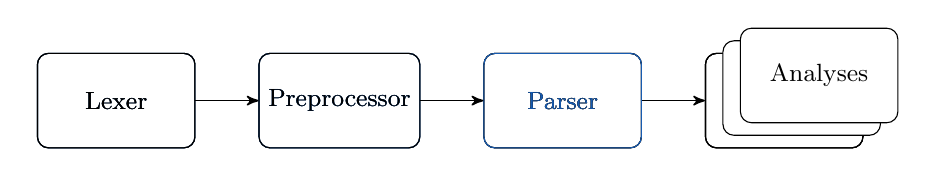
\begin{tikzpicture}
		[basic box/.style = {
			draw,
			shape = rectangle,
			align = center,
			minimum width=2cm,
			minimum height=1.2cm,
			rounded corners
		},
		to/.style = {
			->,
			>=stealth',
			semithick
		},
		every matrix/.style={column sep=.8cm, ampersand replacement=\&},
		font=\small
		]
		\onslide<1>{
			\matrix{
				\node[basic box, {CTUBlue}] (a) {Lexer};
			\&  \node[basic box] (b) {Preprocessor};
			\&  \node[basic box] (c) {Parser};
			\&  \node[basic box] (d) {}; \\
			};
		}
		\onslide<2>{
			\matrix{
				\node[basic box] (a) {Lexer};
			\&  \node[basic box, {CTUBlue}] (b) {Preprocessor};
			\&  \node[basic box] (c) {Parser};
			\&  \node[basic box] (d) {}; \\
			};
		}
		\onslide<3->{
			\matrix{
				\node[basic box] (a) {Lexer};
			\&  \node[basic box] (b) {Preprocessor};
			\&  \node[basic box, {CTUBlue}] (c) {Parser};
			\&  \node[basic box] (d) {}; \\
			};
		}

		\node[basic box, fill=white, above right=-3em and -5.1em of d ] (d2) {};
		\node[basic box, fill=white, above right=-3em and -5.1em of d2] (d3) {Analyses};

		\path
		(a) edge[to] (b)
		(b) edge[to] (c)
		(c) edge[to] (d)
		;
	\end{tikzpicture}
	\end{overprint}
\end{frame}

\begin{frame}{Parsing expression grammars}
	\begin{itemize}
		\item Closely related to context-free grammars \pause
		\item Major difference: \alert{ordered choice} operator \pause
		\item Packrat parsers recognise PEG productions in linear time
	\end{itemize}
\end{frame}

\begin{frame}{Syntax of parsing expression grammars}
	\centering
	\begin{overprint}
	\begin{align*}
		e ::= & \hspace{2pt} \varepsilon & \text{(empty string)} \\
		\mid  & \hspace{2pt} \texttt{t}  & \text{(terminal)} \\
		\mid  & \hspace{2pt} e_1 e_2     & \text{(sequence)} \\
		\mid  & \hspace{2pt} \alert{e_1 | e_2} & \alert{\text{(ordered choice)}} \\
		\mid  & \hspace{2pt} e^*         & \text{(zero or more)} \\
		\mid  & \hspace{2pt} e^+         & \text{(one or more)} \\
		\mid  & \hspace{2pt} e?          & \text{(zero or one)} \\
		\mid  & \hspace{2pt} \alert{\&e} & \alert{\text{(positive lookahead)}} \\
		\mid  & \hspace{2pt} \alert{!e}  & \alert{\text{(negative lookahead)}} \\
		\texttt{t} \in & \hspace{2pt} \text{tokens}
	\end{align*}
	\end{overprint}
\end{frame}

\begin{frame}{Results}
	\begin{itemize}
		\item Proof-of-concept language server for P4 \pause
		\item Integrated with Visual Studio Code \pause
		\item Plugs into other LSP-capable editors \pause
		\item Supports \alert{error-tolerant autocompletion} \pause
		\item Provides diagnostics for preprocessor issues \pause
		\item Features simple go-to definition functionality
	\end{itemize}
\end{frame}

\begin{frame}{Showcase}
	\begin{overprint}
	\only<1> {
		\includegraphics[width=\textwidth]{resources/p4analyzer-autocompletion.png}
	}
	\only<2> {
		\includegraphics[width=\textwidth]{resources/p4analyzer-preprocessor-response.png}
	}
	\only<3> {
		\includegraphics[width=\textwidth]{resources/p4analyzer-preprocessor-errors.png}
	}
	\end{overprint}
\end{frame}

\begin{frame}{Summary}
	\begin{itemize}
		\item LSP-compliant analyser for P4 \pause
		\item Incremental analysis pipeline \pause
		\item Packrat parsing
	\end{itemize}
\end{frame}

\begin{frame}{}
	Thank you for listening.

	\begin{thebibliography}{1}
		\bibitem{thesis}
		Kvapil, Ondřej.
		\textit{P4 Language Server}.
		Master's thesis.
		Czech Technical University in Prague,
		Faculty of Information Technology, 2023.
	\end{thebibliography}

	\url{https://github.com/viluon/masters-thesis}
\end{frame}

\begin{frame}[fragile]{Questions for the defense}
	\alert{
		\begin{overprint}
			\onslide<1-2> Question 1
			\onslide<3-4> Question 2
			\onslide<5-6> Question 3
		\end{overprint}
	}

	\begin{displayquote}
		\begin{overprint}
			\onslide<1-2>
			Did you consider some alternative approaches for the incremental
			parsing? Popular incremental parser is \texttt{treesitter} (although
			I have not seen it used in any LSP I know).

			\onslide<3-4>
			I don't know how large the P4 programs tend to be, but did you look
			at how much the incrementality actually helps?

			\onslide<5-6>
			Did you consider using \texttt{rowan} for the lossless syntax trees?
		\end{overprint}
	\end{displayquote}

	\begin{overprint}
		\onslide<2>
		Yes. \texttt{treesitter} is a generator of incremental parsers with
		high-level features that ease integration with LSP. Unfortunately, it
		relies on character-level access and \alert{is not general over the type
		of tokens}. Integrating it would require lowering preprocessed tokens
		back to text and passing them as a string to the \texttt{treesitter}
		parser, effectively lexing twice and complicating source location
		tracking.
		\\\\
		We wanted to avoid this inefficiency in our design, but switching to
		\texttt{treesitter} is an option for future work.

		\onslide<4>
		Our P4 grammar is only a proof-of-concept, so we cannot yet benchmark
		parsing of practical programs. For the purposes of this defense, I
		\alert{performed an experiment} to investigate incremental performance
		for a simple input with repeated definitions.

		\vspace{0.5cm}

		\begin{tikzpicture}
			\begin{axis}[
				xlabel=Number of definitions,
				ylabel=Run time \lbrack{ms}\rbrack,
				height=4cm,
				width=\textwidth,
				legend pos=north west,
			]
			\addplot[color=orange,mark=square] table [x=Definitions, y={From scratch}]{measurements.dat};
			\addlegendentry{From scratch}

			\addplot[color=CTUBlue,mark=triangle] table [x=Definitions, y=Incremental]{measurements.dat};
			\addlegendentry{Incremental}
			\end{axis}
		\end{tikzpicture}

		\onslide<6>
		Yes. \texttt{rowan} is a general-purpose library for lossless syntax
		trees, built for the Rust Analyzer project. \texttt{rowan} suffers from
		\alert{the same problem as \texttt{treesitter} -- reliance on text
		input}. However, \texttt{rowan} heavily inspired our own design for
		syntax trees, even though we did not adopt any of its code.

		\begin{lstlisting}[
			basicstyle=\small,
			language=Rust,
			tabsize=4,
		]
impl GreenTokenData {
	/// Text of this Token.
	#[inline]
	pub fn text(&self) -> &str {
		unsafe { std::str::from_utf8_unchecked(self.data.slice()) }
	}
}
		\end{lstlisting}
	\end{overprint}
\end{frame}

\end{document}
